\documentclass{article}   

\usepackage{geometry}
\usepackage{qtree}
\usepackage[square,numbers]{natbib}
% \usepackage{cite}  
\geometry{a4paper}

\usepackage[]{algorithm2e}
\usepackage{amsthm}
\newtheorem{theorem}{Theorem}[section]
\newtheorem{corollary}{Corollary}[theorem]
\newtheorem{lemma}[theorem]{Lemma}
\usepackage{rotating}
\usepackage[utf8]{inputenc}
\usepackage[T1]{fontenc}    % use 8-bit T1 fonts
\usepackage{lmodern}
\usepackage{hyperref}       % hyperlinks
\usepackage{lipsum}

%\usepackage[dvipsnames]{xcolor}
\usepackage{color, colortbl}

\definecolor{Gray}{gray}{0.9}
\definecolor{goldenpoppy}{rgb}{0.99, 0.76, 0.0}
\definecolor{goldenrod}{rgb}{0.85, 0.65, 0.13}

\usepackage[protrusion=true,expansion=true]{microtype}

\usepackage{amssymb}
\usepackage{amsfonts}
\usepackage{eqnarray,amsmath}
\usepackage[table]{xcolor}

\usepackage{listings}
\usepackage{graphicx}
\usepackage{dirtytalk}

\usepackage{rotating}
\usepackage{caption}

%% if you use PostScript figures in your article
%% use the graphics package for simple commands
\usepackage{graphics}


%% or use the graphicx package for more complicated commands
\usepackage{graphicx}


\usepackage{indentfirst}
\usepackage[utf8]{inputenc}
 \usepackage{subcaption}

 
\usepackage{xspace,color}
\usepackage{url}

\usepackage[export]{adjustbox}

\lstset{commentstyle=\color{red},keywordstyle=\color{black},
showstringspaces=false}
\lstnewenvironment{rc}[1][]{\lstset{language=R}}{}
\newcommand{\ri}[1]{\lstinline{#1}}  %% Short for 'R inline'

\lstset{language=R}             % Set R to default language


%https://tex.stackexchange.com/questions/96825/nicely-formatted-where-statement-for-maths
 \newenvironment{where}{\noindent{}where\begin{itemize}}{\end{itemize}}
 \renewcommand*\descriptionlabel[1]{\hspace\leftmargin$#1$}
 
\lstset{escapeinside={<@}{@>}}
% please place your own definitions here and don't use \def but
% \newcommand{}{}
%
% Insert the name of "your journal" with
% \journalname{myjournal}
%
\begin{document}

\title{%
  Practice 10: Simulations of expected value and variance of random variables} %\\~\\
  %\Large }
\author{Mayra Cristina Berrones Reyes 6291}

\maketitle

\section{Exercises}

The exercises of this work where taken from the book Introduction to probability by Charles M. Grinstead and J. Laurie Snell \cite{grin}.

\subsection{Exercise 1, page 247}\label{ex1}

A card is drawn at random form a deck consisting of cards numbered from 2 to 10. A player wins 1 dollar if the number on the card is odd and loses 1 dollar if the number is even. What is the expected value of his winnings?\\

\begin{itemize}
\item \textbf{Experimentation:}
\end{itemize}

For this experiment, we used the \texttt{sample} function in \texttt{R}. Inside a loop of 10,000 repetitions, we made a variable that gives us at random a number between 2 and 10. Then we divided the results in even and odd numbers. In Figure \ref{sb1-1} we can see a pie plot of one iteration of the 10,000 repetition of the card experiment. In this case, the red represents the number of times the card was an even number, and the blue represents the odd ones. At first sight we can see that the losses are greater than the winnings. \\

The expected value of this single experiment was $E(X) = -0.116$. The value resembles the result of our analytic experiment. To test it further, we performed 100 iterations of the 10,000 repetitions. In this case, Figure \ref{sb1-2} is the histogram showing how the results are distributed. As we can see, the majority of the experiment land in the range of $-0.12$ and $-0.10$, proving with experimentation, that our analysis was correct.\\

\begin{figure}[]
\begin{subfigure}{.48\textwidth}
  \centering
  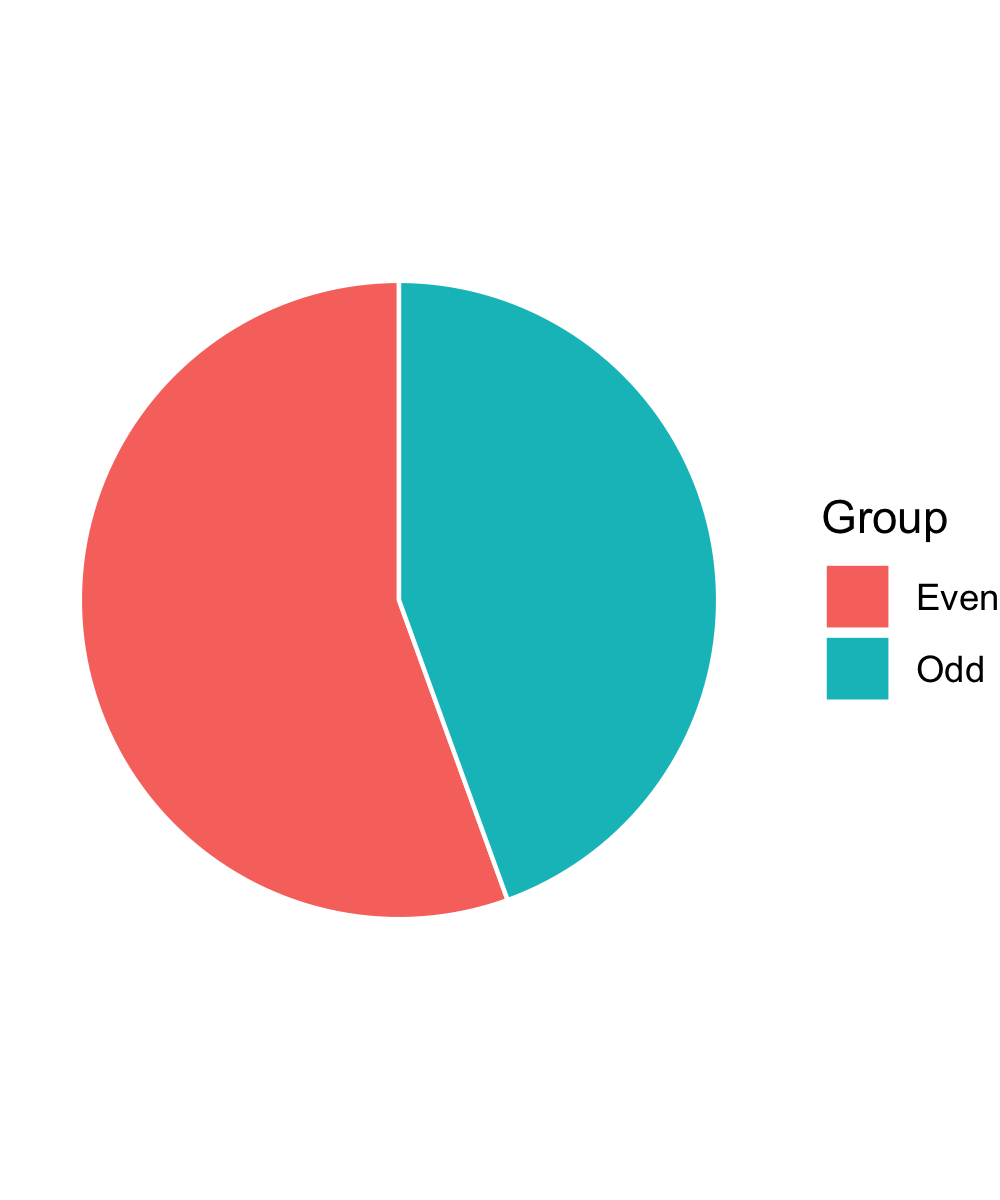
\includegraphics[width=.9\linewidth, left]{Ej10_even.png}  
  \caption{Pie plot of the one iteration of the 10,000 repetitions of the card experiment. }
  \label{sb1-1}
\end{subfigure}\hspace{5mm}%
\begin{subfigure}{.48\textwidth}
  \centering
  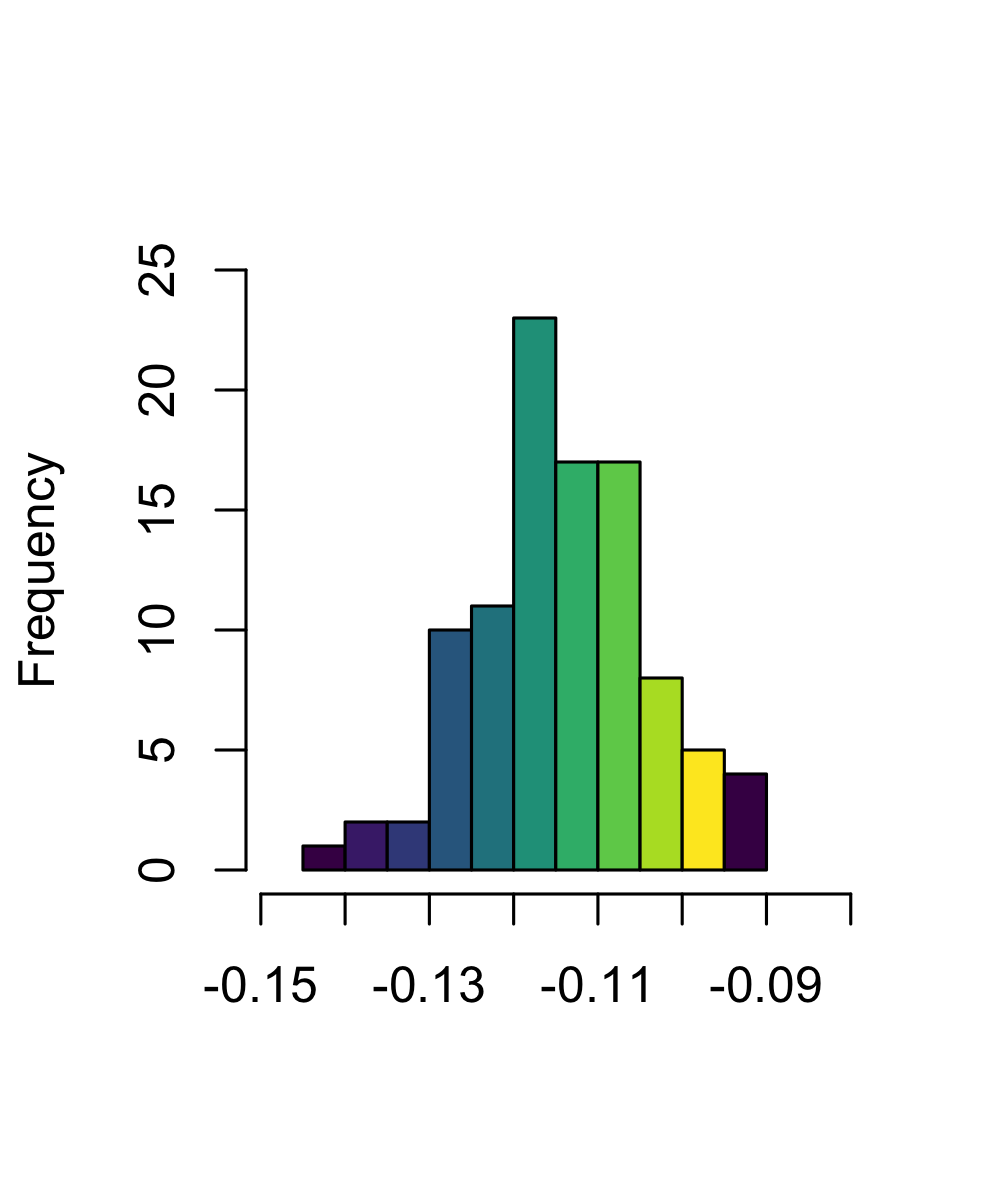
\includegraphics[width=.9\linewidth, right]{Ej10_hist1.png}  
  \caption{Histogram of the 100 iterations of the 10,000 repetitions of the card experiment.}
  \label{sb1-2}
\end{subfigure}
	\caption{Pie plot and histogram of the experiment.}
\label{fig1}
\end{figure}


\begin{flushright}
$\blacksquare$
\end{flushright}

\subsection{Exercise 6, page 247}\label{ex2}

A die is rolled twice. Let $X$ denote the sum of the two numbers that turn up, and $Y$ the difference of the numbers (specifically, the number on the first roll minus the number of the second). Show that $E(XY) = E(X)E(Y)$. Are $X$ and $Y$ independent?\\

 \begin{table}[]\caption{Calculation of probabilities for the expected value of $X$.}\label{tab1}
\centering
\begin{tabular}{| p{2cm} | c | c | c | c | c | c | c | c | c | c | c |}
\hline
$X$ value & 2 & 3 & 4 & 5 & 6 & 7 & 8 & 9 & 10 & 11 & 12 \\
\hline 
Probabilities of each one & $\frac{1}{36}$& $\frac{2}{36}$& $\frac{3}{36}$& $\frac{4}{36}$& $\frac{5}{36}$& $\frac{6}{36}$& $\frac{5}{36}$& $\frac{4}{36}$& $\frac{3}{36}$& $\frac{2}{36}$& $\frac{1}{36}$\\
\hline 
Simplifying fractions& $\frac{1}{36}$& $\frac{1}{18}$& $\frac{1}{12}$& $\frac{1}{9}$& $\frac{5}{36}$& $\frac{1}{6}$& $\frac{5}{36}$& $\frac{1}{9}$& $\frac{1}{12}$& $\frac{1}{18}$& $\frac{1}{36}$\\
\hline
\end{tabular}
\end{table}



 \begin{table}[]\caption{Calculation of probabilities for the expected value of $Y$.}\label{tab2}
\centering
\begin{tabular}{| p{2cm} | c | c | c | c | c | c | c | c | c | c | c |}
\hline
$Y$ value & 0 & -1 & -2 & -3 & -4 & -5 & 1 & 2 & 3 & 4 & 5 \\
\hline 
Probabilities of each one & $\frac{1}{36}$& $\frac{5}{36}$& $\frac{4}{36}$& $\frac{3}{36}$& $\frac{2}{36}$& $\frac{1}{36}$& $\frac{5}{36}$& $\frac{4}{36}$& $\frac{3}{36}$& $\frac{2}{36}$& $\frac{1}{36}$\\
\hline 
Simplifying fractions& $\frac{1}{6}$& $\frac{5}{36}$& $\frac{1}{9}$& $\frac{1}{12}$& $\frac{1}{18}$& $\frac{1}{36}$& $\frac{5}{36}$& $\frac{1}{9}$& $\frac{1}{12}$& $\frac{1}{18}$& $\frac{1}{36}$\\
\hline
\end{tabular}
\end{table}


 \begin{table}[]\caption{Calculation of probabilities for the expected value of $XY$.}\label{tab3}
\centering
\begin{tabular}{| p{2cm} | c | c | c | c | c | c | c | c | c | c | c | c | }
\hline
$XY$ value & 0 & -3 & -8 & -15 &-24 & -35 & 3 & -5 & -12 & -21 & -32 & 8  \\
\hline 
Probabilities of each one & $\frac{6}{36}$& $\frac{1}{36}$& $\frac{1}{36}$& $\frac{1}{36}$& $\frac{1}{36}$& $\frac{1}{36}$& $\frac{1}{36}$& $\frac{1}{36}$& $\frac{1}{36}$& $\frac{1}{36}$& $\frac{1}{36}$& $\frac{1}{36}$\\
\hline
\hline
$XY$ value & 5 & -7 & -16 & -27 &15 & 12 & 7 & -9 & -20 & 24 & 21 & 16  \\
\hline 
Probabilities of each one & $\frac{1}{36}$& $\frac{1}{36}$& $\frac{1}{36}$& $\frac{1}{36}$& $\frac{1}{36}$& $\frac{1}{36}$& $\frac{1}{36}$& $\frac{1}{36}$& $\frac{1}{36}$& $\frac{1}{36}$& $\frac{1}{36}$& $\frac{1}{36}$\\
\hline
\hline
$XY$ value & 9 & -11 & 35 & 32 &27 & 20 & 11 &  &  &  &  &   \\
\hline 
Probabilities of each one & $\frac{1}{36}$& $\frac{1}{36}$& $\frac{1}{36}$& $\frac{1}{36}$& $\frac{1}{36}$& $\frac{1}{36}$& $\frac{1}{36}$& & & & & \\
\hline
\end{tabular}
\end{table}



\begin{itemize}
\item \textbf{Experimentation:}
\end{itemize}

In this case, we replicated the experiment made in Exercise \ref{ex1}. In Figure \ref{sb2-1}, \ref{sb2-2}, and \ref{sb2-3} we can see a pie plot with only one experimentation of each expected value experiment. If we compare the results we have from Table \ref{tab1}, \ref{tab2} and \ref{tab3} we can see that the distribution in the pie plot resembles our analitical results. \\

\begin{figure}[]
\begin{subfigure}{.5\textwidth}
  \centering
  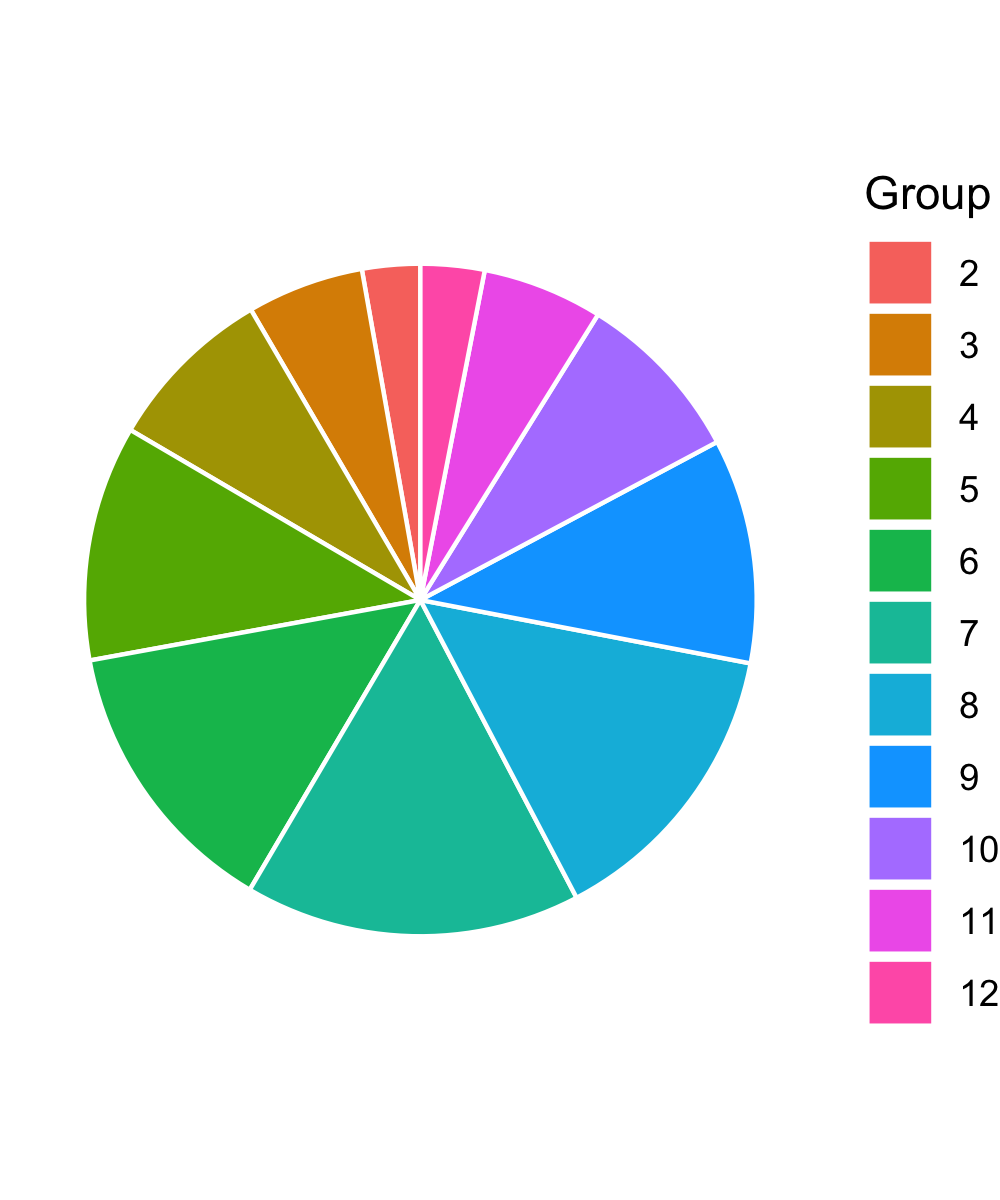
\includegraphics[width=1\linewidth, left]{Ej10_pie1.png}  
  \caption{Pie plot of the one iteration of the 10,000 repetitions of the dice experiment for $E(X)$. }
  \label{sb2-1}
\end{subfigure}\hspace{5mm}%
\begin{subfigure}{.5\textwidth}
  \centering
  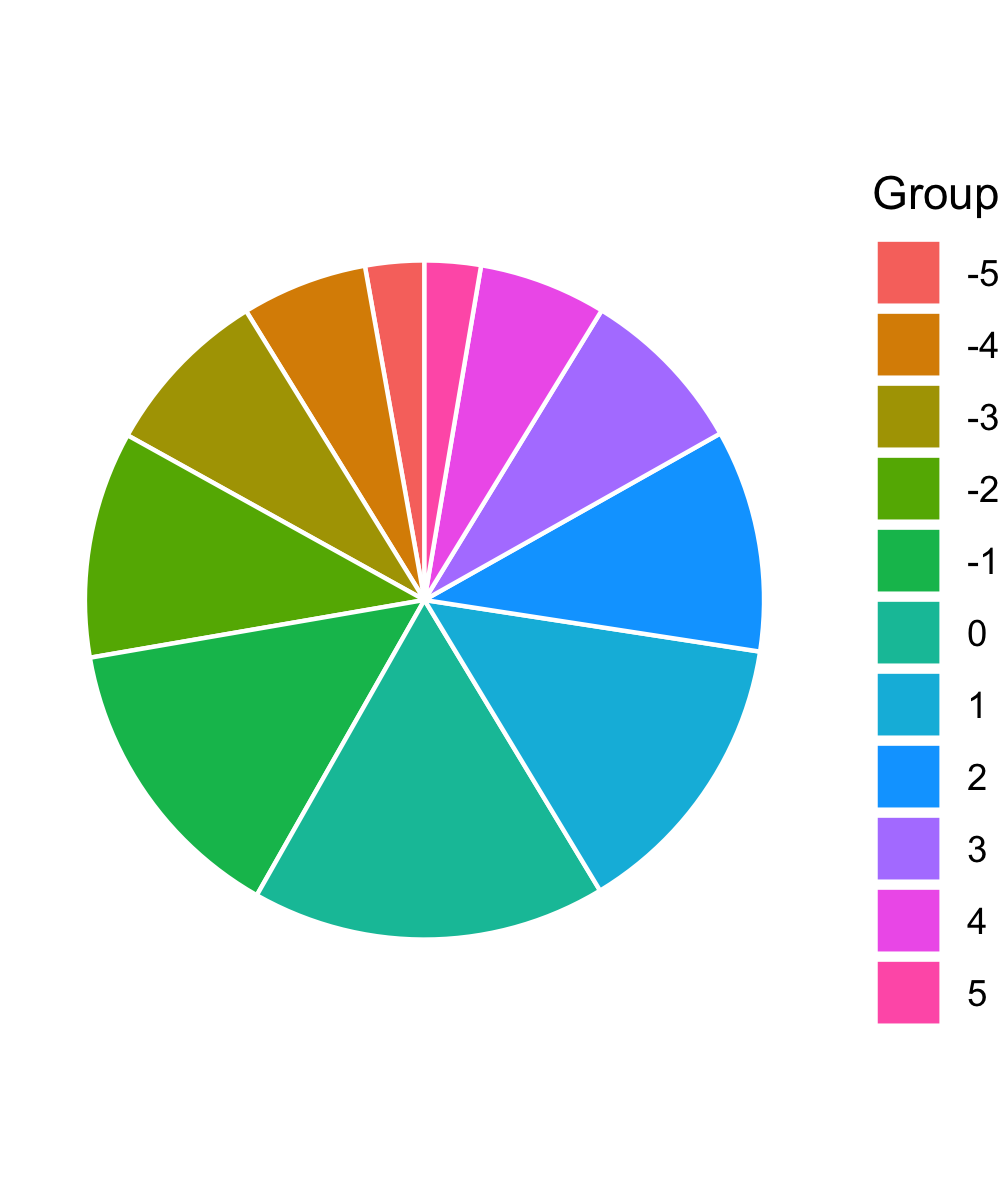
\includegraphics[width=1\linewidth]{Ej10_pie2.png}  
  \caption{Pie plot of the one iteration of the 10,000 repetitions of the dice experiment for $E(Y)$. }
  \label{sb2-2}
\end{subfigure}\hspace{5mm}%
\newline
\begin{subfigure}{1\textwidth}
  \centering
  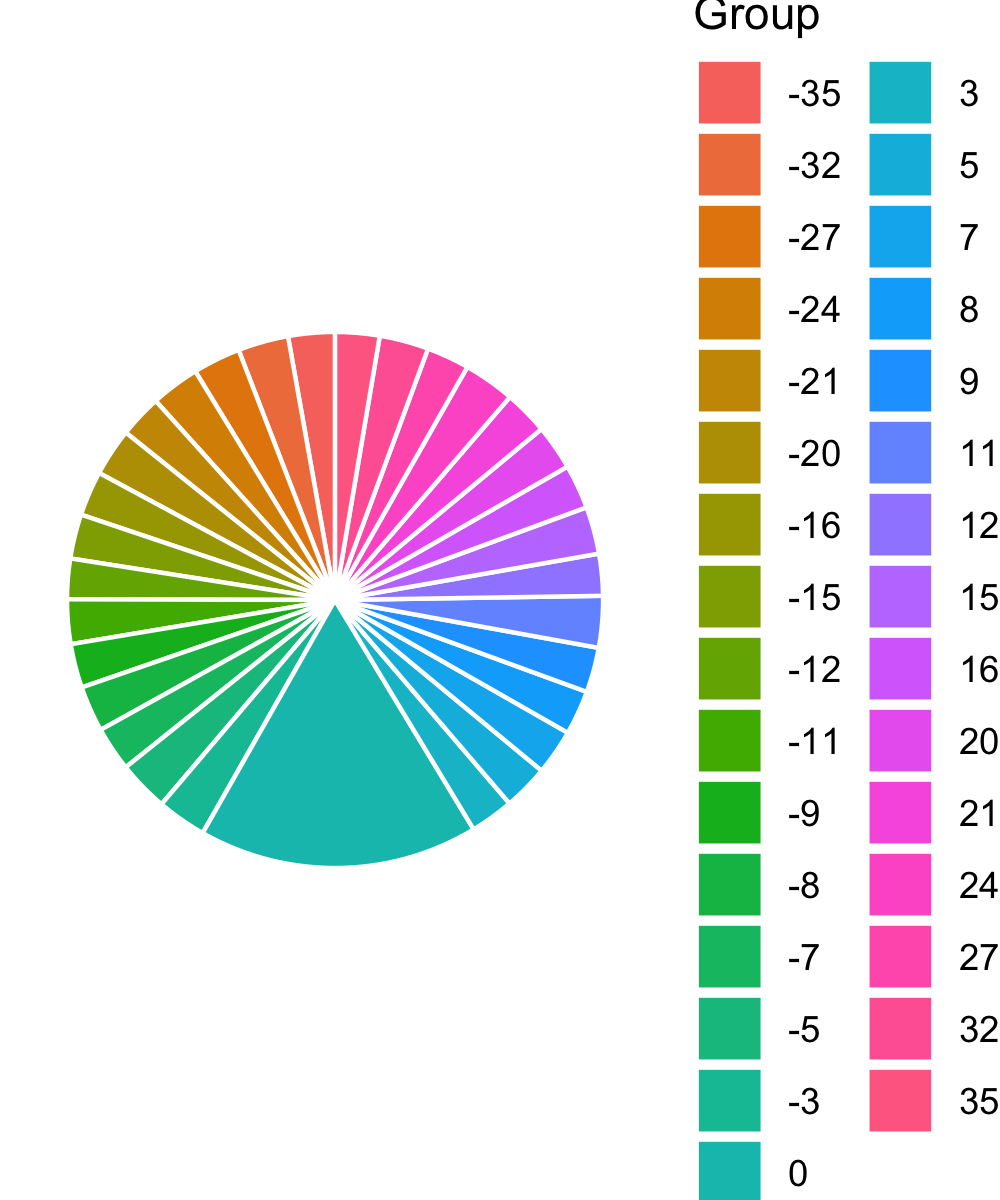
\includegraphics[width=.5\linewidth]{Ej10_pie3.png}  
  \caption{Pie plot of the 100 iterations of the 10,000 repetitions of the dice experiment for $E(XY)$.}
  \label{sb2-3}
\end{subfigure}
	\caption{Pie plot of the different expected values of the experiment.}
\label{fig2}
\end{figure}

Keeping with the example of Exercise \ref{ex1} we then made an experimentation of 100 iterations of 10,000 repetitions of the same experiment, to see if the result behaves like we expected. In Figure  \ref{fig3} we have the histograms of each expected value. \\

In Figure \ref{sb3-1} we have the experiment for $E(X)$ and according to our analysis, the result should be 7. The histogram clearly shows a majority of the distribution in a range of $6.90$ to $7.05$, so our calculation can be deemed correct. In Figure \ref{sb3-2} we have the experiment of the $E(Y)$. Here the result is 0 in our analysis, and as we can see, the interval of the distribution for the results is from $-0.06$ to $0.06$, so we can again say our analysis is correct. Lastly for Figure \ref{sb3-3} we have the experimentation for the $E(XY)$. Here the result should also be $0$ according to our analysis. In this case, the interval is a bit more wide, but the majority of the distribution on this histogram still focuses on $-0.2$ to $0.2$

\begin{figure}[]
\begin{subfigure}{.3\textwidth}
  \centering
  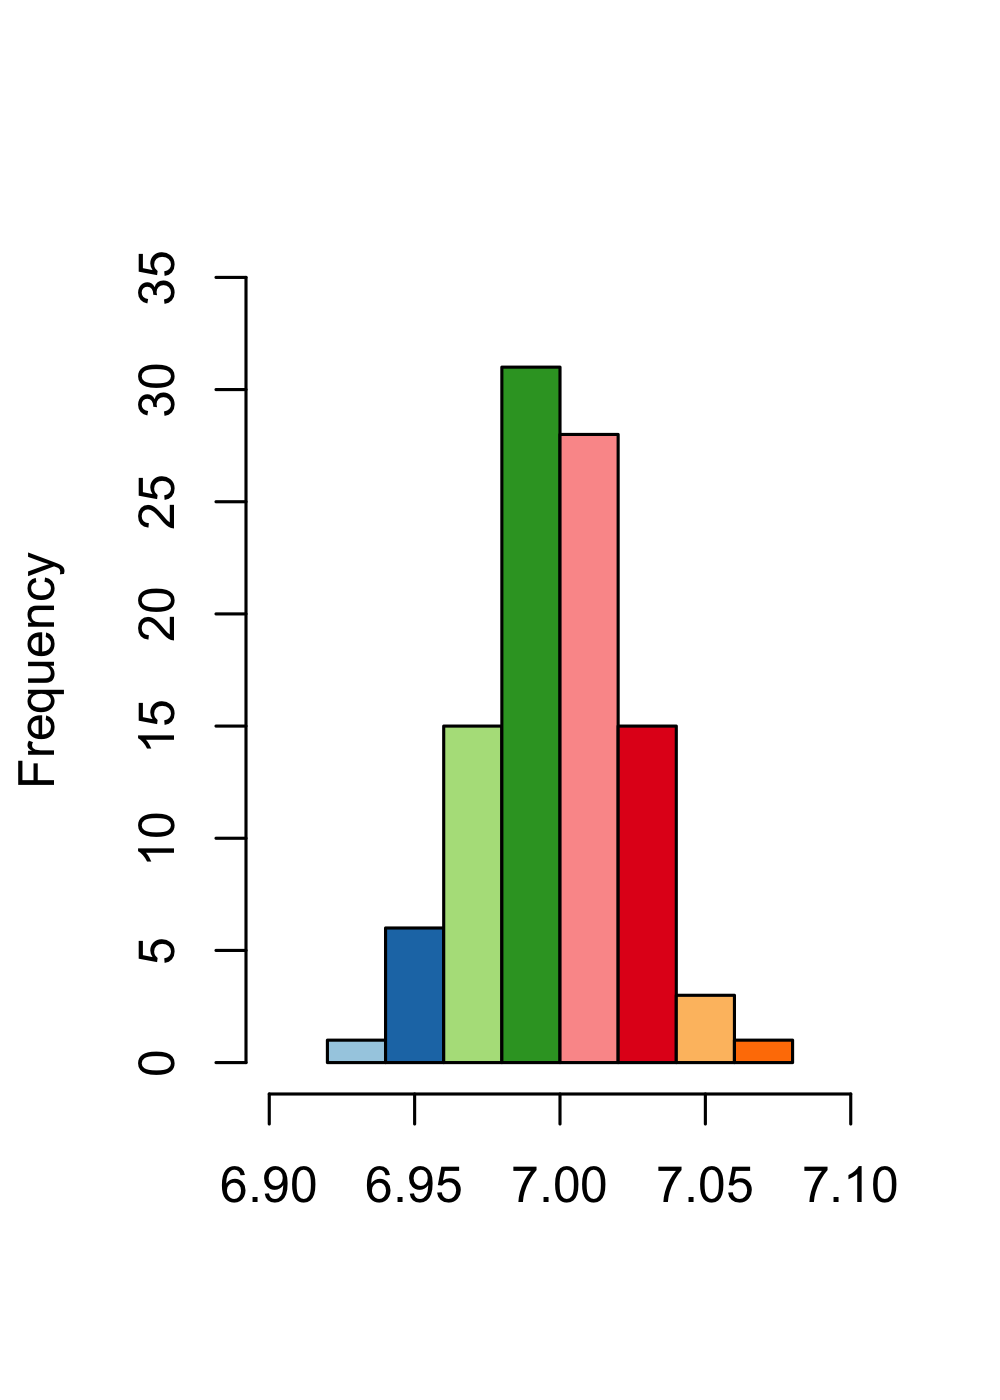
\includegraphics[width=1\linewidth, left]{Ej10_hist2.png}  
  \caption{Histogram of the dice experiment for $E(X)$. }
  \label{sb3-1}
\end{subfigure}\hspace{5mm}%
\begin{subfigure}{.3\textwidth}
  \centering
  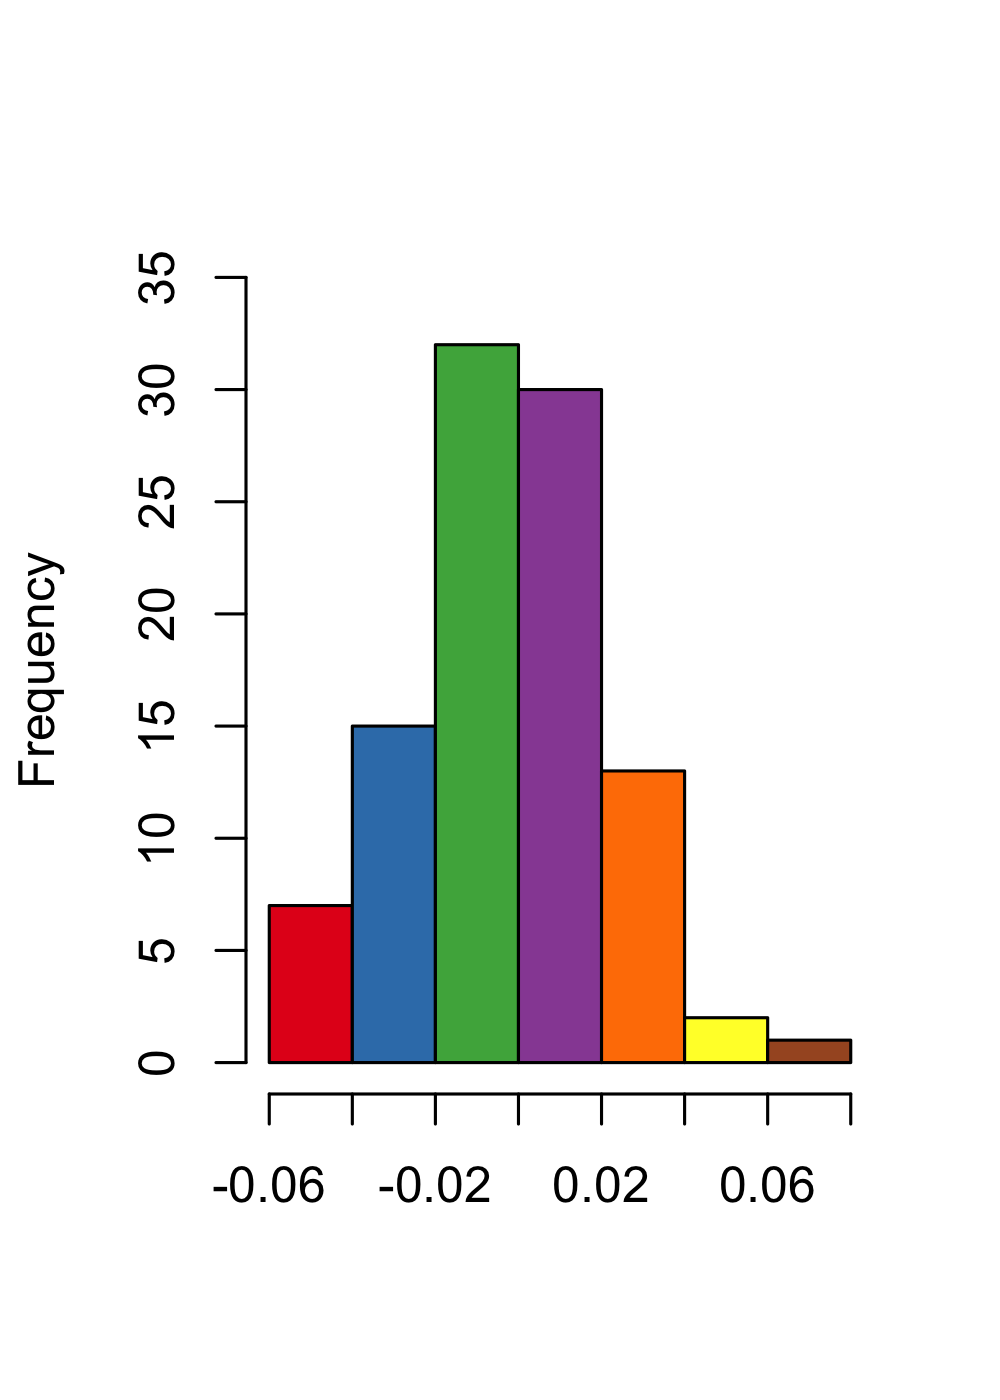
\includegraphics[width=1\linewidth]{Ej10_hist3.png}  
  \caption{Histogram of the dice experiment for $E(Y)$. }
  \label{sb3-2}
\end{subfigure}\hspace{5mm}%
\begin{subfigure}{.3\textwidth}
  \centering
  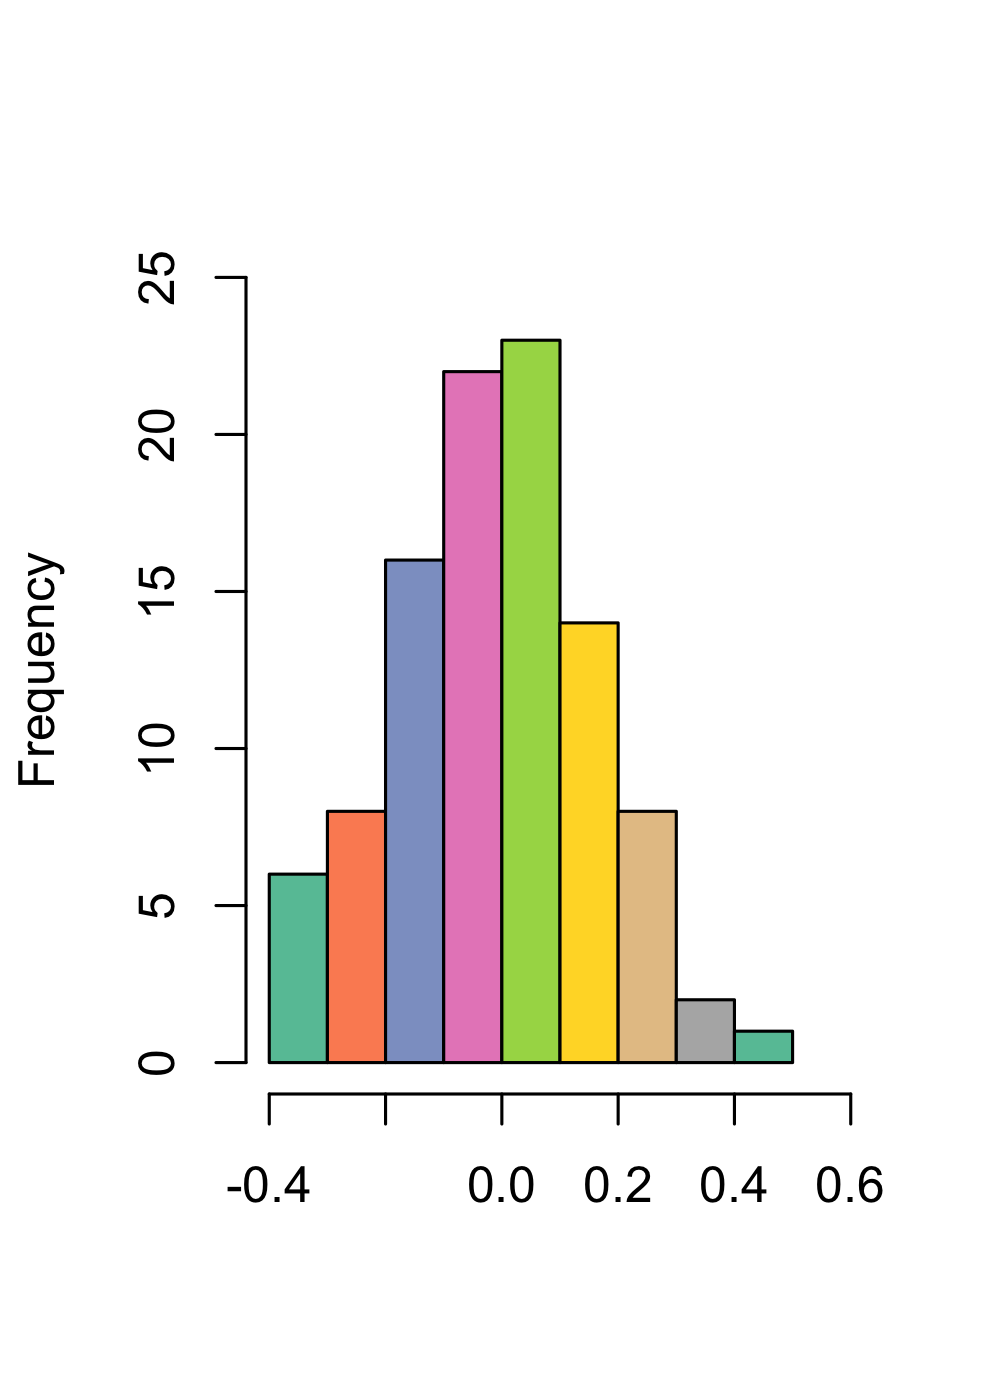
\includegraphics[width=1\linewidth, right]{Ej10_hist4.png}  
  \caption{Histogram of the dice experiment for $E(XY)$.}
  \label{sb3-3}
\end{subfigure}
	\caption{Histograms of the 100 iterations of the 10,000 repetitions from the expected value of all the experiments.}
\label{fig3}
\end{figure}
 
\begin{flushright}
$\blacksquare$
\end{flushright}


\subsection{Exercise 15, page 249}

A box contains two gold balls and three silver balls. You are allowed to choose successively from the box at random. You win 1 dollar each time you draw a gold ball and lose 1 dollar each time you draw a silver ball. After a draw, the ball is not replaced. Show that, if you draw until you are ahead by 1 dollar, or until there are no more gold balls, this is a favorable game.\\

\begin{itemize}
\item \textbf{Experimentation:}
\end{itemize}

For this experimentation, first we replicated the rules that the exercise dictates. In \texttt{R} we used the library \texttt{arrangements} to make the different scenarios of drawing the balls. Table \ref{tb4} gives us the result of this library. We represented the golden and silver balls according to their colors, and the value they give us when we draw them. The las column called winnings represents the final result, following the rules of ending the game if we are ahead by 1 dollar, or if we draw both silver balls.\\

In Figure \ref{fig4} we have the graphical representation of the the experiment, in which we draw a different configuration 10,000 times. The problem asks us to prove that if we draw until we are ahead by one dollar or there are no more gold balls, that the resulting winnings are still a favorable game. In our analysis we concluded that, if we count as a favorable result when we end up without losses nor winnings, $\frac{7}{10}$ of the times, we end up with favorable results. \\

In the experiment of 10,000 we have that 0.7059 of the times, we have a favorable result, proving our analysis correct.\\
 
 \begin{table}[]\caption{Different resulting winnings on the different scenarios}\label{tb4}
\centering
\begin{tabular}{ r  r  r  r  r  r  r  }
 &( ,1) & ( ,2) &( ,3) &( ,4) &( ,5) & Winnings \\
(1, )  & \textbf{\color{gray}{-1}} & \textbf{\color{gray}{-1}} &\textbf{\color{gray}{-1}} &\textbf{\color{goldenrod}{1}} & \textbf{\color{goldenrod}{1}}& -1\\
(2, )& \textbf{\color{gray}{-1}} & \textbf{\color{gray}{-1}} &\textbf{\color{goldenrod}{1}} & \textbf{\color{gray}{-1}} & \textbf{\color{goldenrod}{1}}& -1\\
(3, ) &  \textbf{\color{gray}{-1}}&  \textbf{\color{gray}{-1}}&\textbf{\color{goldenrod}{1}} & \textbf{\color{goldenrod}{1}}& \textbf{\color{gray}{-1}}& 0\\
(4, ) & \textbf{\color{gray}{-1}} & \textbf{\color{goldenrod}{1}} & \textbf{\color{gray}{-1}}& \textbf{\color{gray}{-1}}& \textbf{\color{goldenrod}{1}}& -1\\
(5, ) & \textbf{\color{gray}{-1}} &  \textbf{\color{goldenrod}{1}}& \textbf{\color{gray}{-1}} &\textbf{\color{goldenrod}{1}} & \textbf{\color{gray}{-1}}& 0\\
(6, ) & \textbf{\color{gray}{-1}} & \textbf{\color{goldenrod}{1}} & \textbf{\color{goldenrod}{1}}& \textbf{\color{gray}{-1}}& \textbf{\color{gray}{-1}}& 1\\
(7, ) & \textbf{\color{goldenrod}{1}} & \textbf{\color{gray}{-1}} &\textbf{\color{gray}{-1}} &\textbf{\color{gray}{-1}} & \textbf{\color{goldenrod}{1}}& 1\\
(8, ) &  \textbf{\color{goldenrod}{1}}& \textbf{\color{gray}{-1}} &\textbf{\color{gray}{-1}} & \textbf{\color{goldenrod}{1}}& \textbf{\color{gray}{-1}}& 1\\
(9, )& \textbf{\color{goldenrod}{1}} &  \textbf{\color{gray}{-1}}&\textbf{\color{goldenrod}{1}} & \textbf{\color{gray}{-1}}& \textbf{\color{gray}{-1}}& 1\\
(10, ) & \textbf{\color{goldenrod}{1}} & \textbf{\color{goldenrod}{1}} & \textbf{\color{gray}{-1}}& \textbf{\color{gray}{-1}}&\textbf{\color{gray}{-1}} &1 \\
\end{tabular}
\end{table}

\begin{figure}[]
\begin{subfigure}{.5\textwidth}
  \centering
  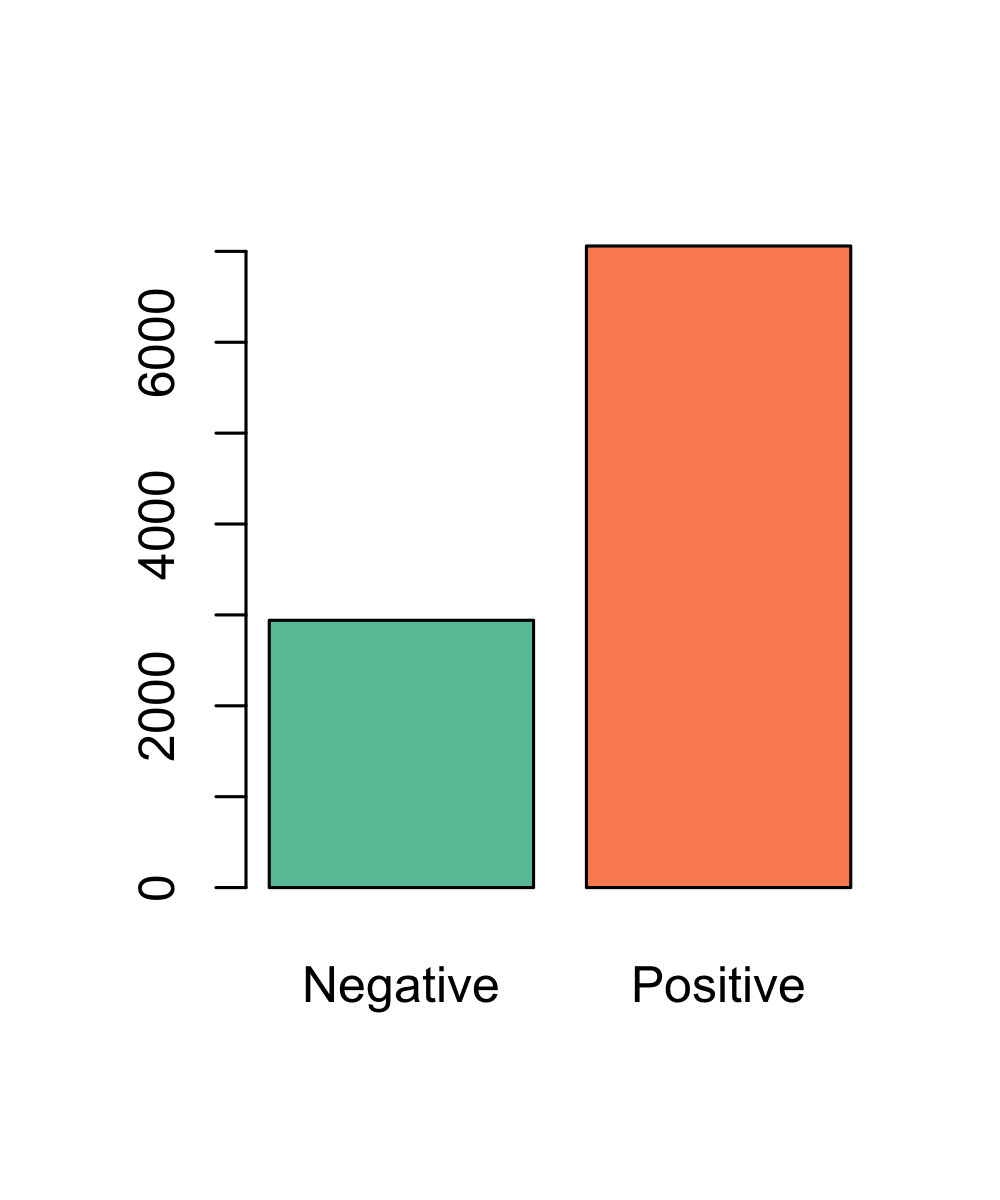
\includegraphics[width=.9\linewidth, left]{Ej10_barplot1.png}  
  \caption{Bar plot of the positive and negative outcomes of the experiment. }
  \label{sb4-1}
\end{subfigure}\hspace{5mm}%
\begin{subfigure}{.5\textwidth}
  \centering
  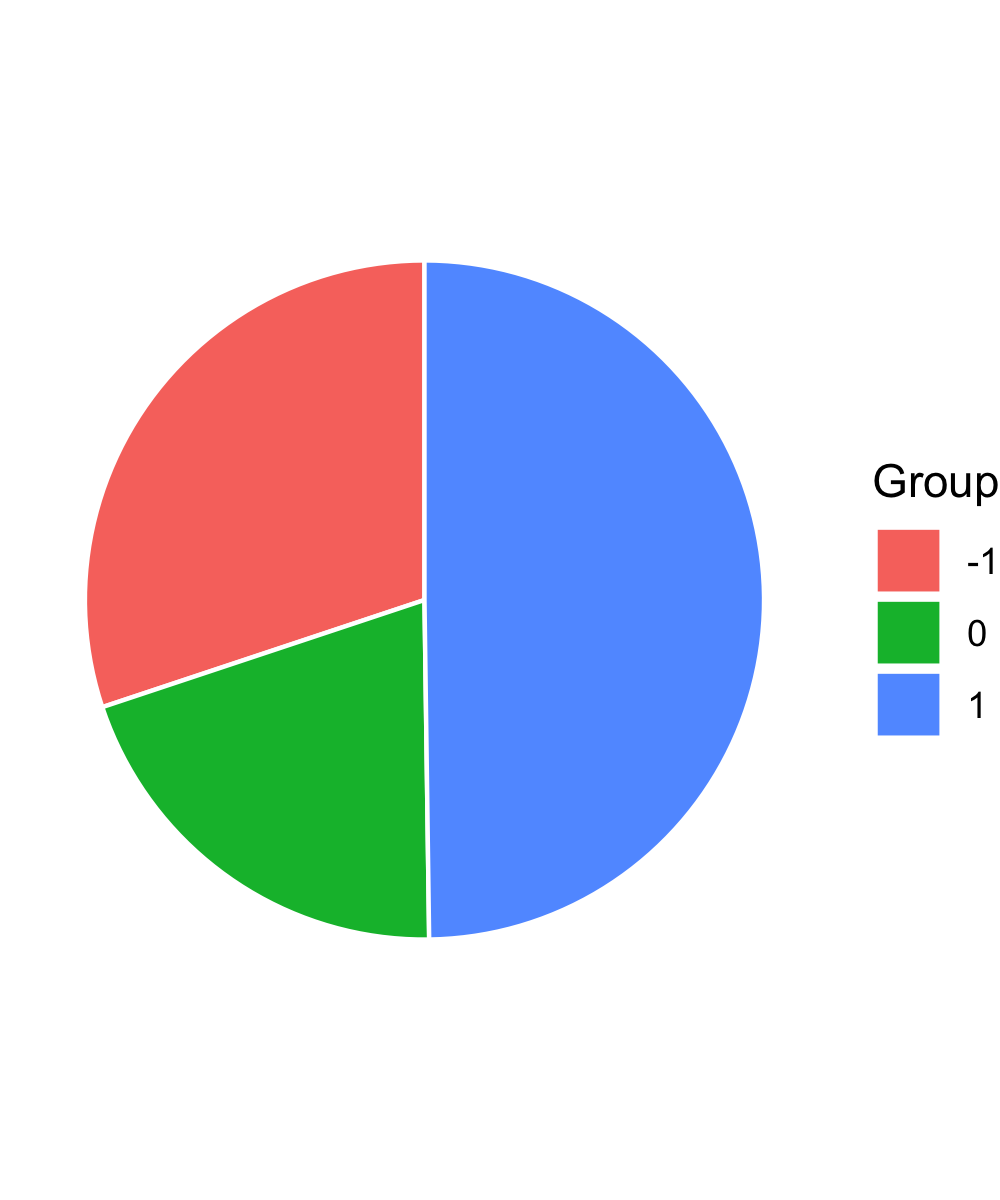
\includegraphics[width=.9\linewidth, right]{Ej10_pie4.png}  
  \caption{Pie plot of the distribution of the different results of the experiment (-1, 0 and 1).}
  \label{sb4-2}
\end{subfigure}
	\caption{Graphic representation of the 10,000 repetition of the experiment. }
\label{fig4}
\end{figure}

\begin{flushright}
$\blacksquare$
\end{flushright}

\subsection{Exercise 18, page 249 (Extra)}

Exactly one of six similar keys opens a certain door. If you try the keys, one after another, what is the expected number of keys that you will have to try before success?\\


\begin{itemize}
\item \textbf{Experimentation:}
\end{itemize}

For this exercise, we used again the library of \texttt{sample}. We selected at random a number between 1 and 6, for a 10,000 repetitions. This number was the correct key. We then checked how many tries it took to find the right key. All these tries where saved in another variable. Using the \texttt{mean} option in \texttt{R} we calculated a mean of 2.4849. \\

In Figure \ref{sb5-1} we have the box plot of one iteration of 10,000 repetitions. The mean in this plot goes to 2, because we used integer numbers, and in the experiment, we can not draw half a key. In Figure \ref{sb5-2} we can see the histogram where we made 100 iterations of the 10,000 repetitions. The interval of medians is between 2.44 to 2.54, being the majority of the frequency in the 2.5 mark.\\

\begin{figure}[]
\begin{subfigure}{.5\textwidth}
  \centering
  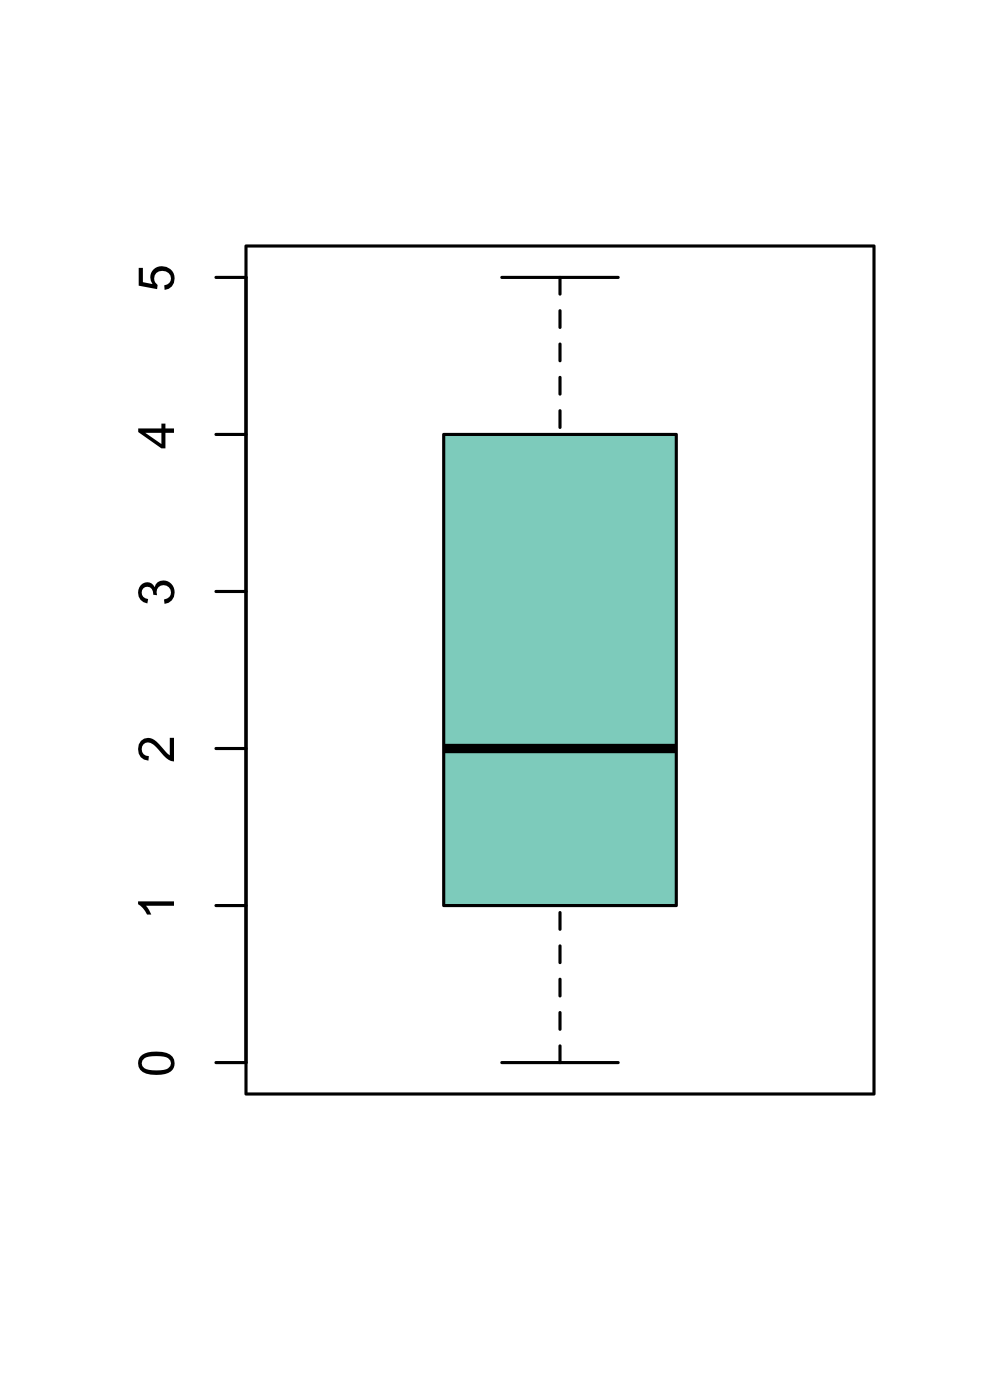
\includegraphics[width=.9\linewidth, left]{Ej10_boxplot1.png}  
  \caption{Box plot of one iteration of 10,000 repetitions. }
  \label{sb5-1}
\end{subfigure}\hspace{5mm}%
\begin{subfigure}{.5\textwidth}
  \centering
  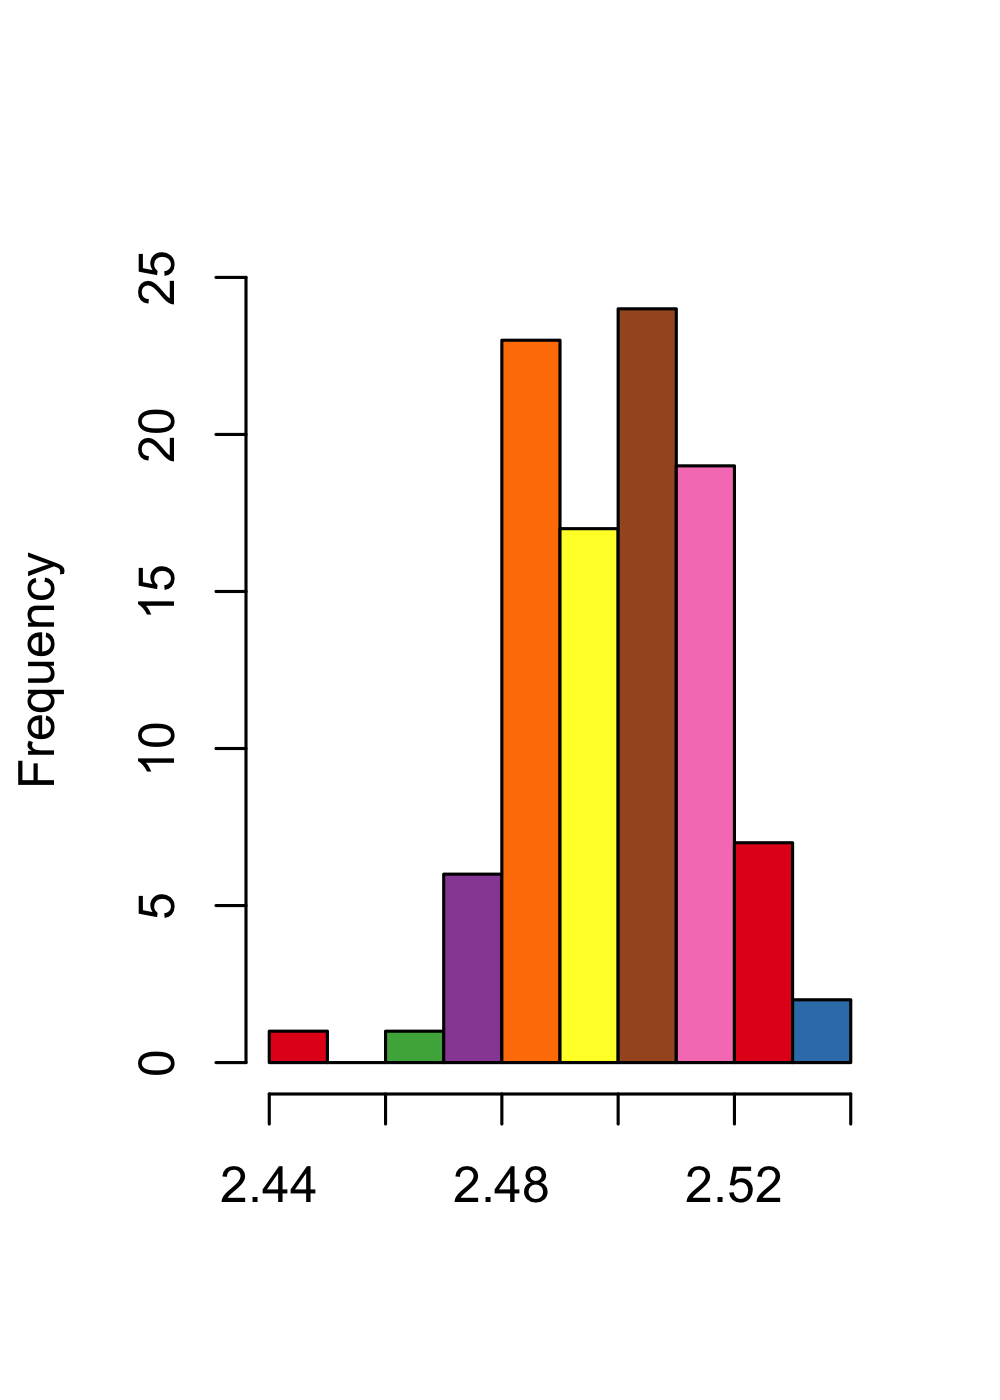
\includegraphics[width=.9\linewidth, right]{Ej10_hist5-1.png}  
  \caption{Histogram of the 100 iterations of the 10,000 repetitions.}
  \label{sb5-2}
\end{subfigure}
	\caption{Graphic representation of the keys experiment. }
\label{fig5}
\end{figure}

\begin{flushright}
$\blacksquare$
\end{flushright}


\subsection{Exercise 27, page 252 (Extra)}
 
 It has been said that a Dr. B. Muriel declined a cup of tea stating that she preferred a cup into which milk had been poured first. The famous statician R. A. Fisher carried out an experiment to see if she could tell whether milk was poured in before or after the tea. Assume that for the test Dr. Bristol was given 8 cups of tea, four in which the milk had been poured before the tea, and four in which the milk was put in after the tea.\\
 
 a) What is the expected number of correct guesses the lady would make if she had no information after each test and was just guessing.
 
 
 \begin{itemize}
\item \textbf{Experimentation:}
\end{itemize}

This is just half of the experimentation, because since Practice 9 I started with some of the analysis of this problem, and I found it kind of funny that these staticians had such an important discovery in probability from an argument about how much do they know of tea. In this case, after some investigation, we found out that Fisher, the one who posed the argument, was so adamant to show that he was right, that he calculated how many cups of tea could Muriel guess correctly if she was in fact just guessing. The proposed hypothesis then was that if she managed to guess all 8, then she indeed must know something about the taste of the tea composition.\\

For this experimentation, we used the \texttt{dhyper} function in \texttt{R} to fill all the information we had about the problem. In this case, we discovered that the chance of Dr. B. Muriel to guess all 8 of them correctly if she was just guessing, was of \textbf{0.013}. In Figure \ref{fig9} we can see the declining probability if the experiment where to continue. After the 14 cup, the probability becomes 0.\\

As a conclusion to this problem, I say that if she managed to guess correctly all of the cups, then she must really know something about the tea. \\

\begin{figure}[]
  \centering
  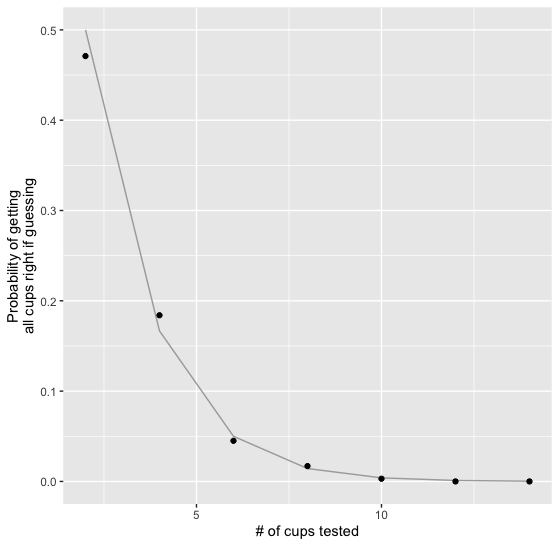
\includegraphics[width=.9\linewidth]{Rplot07.png}  
	\caption{Graphic representation of the diminishing probability of guessing correctly different number of cups }
\label{fig9}
\end{figure}

\begin{flushright}
$\blacksquare$
\end{flushright}

\section{Conclusion}

In this practice, it was easier to develop the experimentation, because we already had the outcome in mind. As a side note, the last extra experiment was a fun conversation in dinner with my family, because now my mother claims she can tell the same difference but with coffee.\\

\bibliographystyle{plainnat}
\bibliography{tarea10}


 
\end{document}